\subsection{Tool Selection}

\subsubsection{Git \& GitHub}
Git is an extremely fast, efficient and distributed version control system ideal for the collaborative development of software. It can be used to manage all your public and private repositories, and makes it easy to share and work with the same source code and documents \cite{bib:git}. GitHub is a hosting system that implements git and is free to use if you choose to share your source code with others. 

\subsubsection{Google Docs}
Google Docs is a free web based service that offers users the ability to create and edit documents online. Google Docs lets us share documents easily and collaborate on the same document simultaneously.    

\subsubsection{NetBeans IDE}
NetBeans IDE is an integrated development environment for developing with Java. It is written in Java and can run on Windows, Linux and OS X. NetBeans IDE is one of the most popular IDEs. Using a common IDE helps speed up the development process.

\subsubsection{Apache Maven}
Maven is a build automation tool which is typically used with Java projects. It uses an XML file to describe the project, the project dependencies on other external modules and components, the build order, directories, and required plug-ins.   

\subsubsection{JIRA with GreenHopper extension}
JIRA is an issue tracking system developed by Atlassian that is used for bug tracking, issue tracking and project management. When used along with the GreenHopper extension it adds support for agile development.

\subsubsection{LaTeX}
LaTeX is a document markup language and document preparation system for the TeX typesetting program. LaTeX was chosen because of the high quality of typesetting that TeX provides.

\subsection{Organizational demands}
There are no organizational demands from Thales, but we agreed on a Scrum based approach. We decided that Scrum is a good lifecycle-model to use since it gives us a runnable product early that can be commented on during the project. This is a pilot project and the specifications are not fully completed, so many revisions are anticipated.

\subsection{Resources}
We are a very diverse group which can go both ways: in our favor and against it. We are all students working on a master's degree in computer science, but the programming experience of each member varies. Two of the group members have
programmed since they were about thirteen years old, while the rest started when they came to NTNU. All of us have at some point had a programming job, and are therefore used to working in teams.
\newline
\newline
Luckily, one might say, we all have different interests regarding what we would like to contribute with. While we agree that we all have to take our part of the programming, documentation and the report work, we can make use of our special interests. As one of us likes to do documentation, another the report work and one of us has much experience in the setup of programming related tasks, we all have gotten our main roles accordingly.
\newline
\newline
Having a group consisting of people with different personalities gives us a challenging group dynamic. By having a daily stand up where everyone shares what they have done, what they will do and what they need to get it done, we are able to get a common understanding of what needs to be done and everyone can get in sync.

\subsection{Schedule of results}

\subsubsection*{Milestones}
See table \ref{tab:milestones} at page \pageref{tab:milestones}
\begin{table}
\begin{tabular}{l|l} \hline
Project start &  21.08.2012\\ 
Pre-delivery of project report & 14.10.2012\\ 
Final delivery of project report & 22.11.2012\\
Project presentation and demonstration & 22.11.2012\\ \hline
\end{tabular}
\caption{Milestones} \label{tab:milestones}
\end{table}

\subsubsection*{Sprints}
See table \ref{tab:sprints} at page \pageref{tab:sprints}
\begin{table}
\begin{tabular}{l|l} \hline
Sprint 1 &  27.08.2012 - 16.09.2012\\
Sprint 2 & 17.09.2012 - 07.10.2012\\
Sprint 3 & 08.10.2012 - 28.10.2012\\
Sprint 4 & 29.10.2012 - 18.11.2012\\ \hline
\end{tabular}
\caption{Sprints} \label{tab:sprints}
\end{table}

\begin{figure}[htb]
\begin{center}
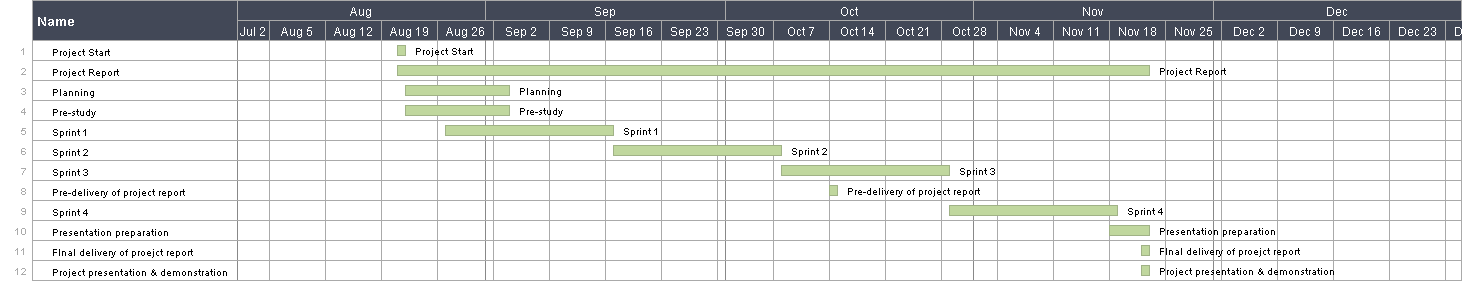
\includegraphics[width=\textwidth, height=2.5in]{foo}
\caption{Gantt-diagram for the entire project}
\end{center}
\end{figure}